\ifdefined\pdfoutput
  \ifnum\pdfoutput=0 \def\pgfsysdriver{pgfsys-dvisvgm.def}\fi
\fi
\documentclass[tikz,border=8pt]{standalone}
\usepackage{amsmath,amssymb}
\usetikzlibrary{arrows.meta}
\begin{document}
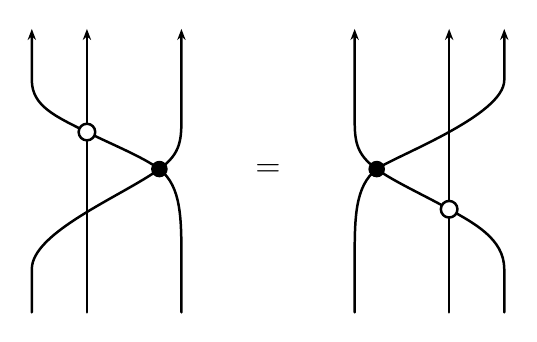
\begin{tikzpicture}[font=\large,line width=.9pt,line cap=round,line join=round,>={Stealth[length=4pt]}]

% Shared editable braid and Kauffman bracket geometry.
% Every primitive accepts optional scale followed by x,y.
% One cubic per full strand: x(t)=a+(b-a)(3t^2-2t^3),
% y(t)=h(1-2t). Endpoint tangents are vertical; reflection swaps strands.
% The white underpass clearance is clipped to the central crossing, so that
% it cannot erase a connection at an endpoint. Width = four structural strokes.
\newcommand{\abaCrossingPaths}[3]{%
  \draw (#2,#3) .. controls (#2,{#3/3}) and (#1,{-#3/3}) .. (#1,{-#3});
  \begin{scope}
    \pgfmathsetmacro{\abacrossradius}{min(abs(#2-#1)/3,#3/2)}
    \clip ({(#1+#2)/2},0) circle (\abacrossradius);
    \draw[white,line width=3.6pt] (#1,#3) .. controls (#1,{#3/3}) and (#2,{-#3/3}) .. (#2,{-#3});
  \end{scope}
  \draw (#1,#3) .. controls (#1,{#3/3}) and (#2,{-#3/3}) .. (#2,{-#3});}
\newcommand{\positivecross}[3][1]{\begin{scope}[shift={(#2,#3)},scale=#1]
\abaCrossingPaths{.42}{-.42}{.62}
\end{scope}}
\newcommand{\negativecross}[3][1]{\begin{scope}[shift={(#2,#3)},scale=#1,xscale=-1]
\abaCrossingPaths{.42}{-.42}{.62}
\end{scope}}
\newcommand{\identitydiagram}[3][1]{\begin{scope}[shift={(#2,#3)},scale=#1]
\draw (-.42,.62)--(-.42,-.62);
\draw (.42,.62)--(.42,-.62);
\end{scope}}
\newcommand{\cupcap}[3][1]{\begin{scope}[shift={(#2,#3)},scale=#1]
\draw (-.42,.62) arc[start angle=180,end angle=360,radius=.42];
\draw (-.42,-.62) arc[start angle=180,end angle=0,radius=.42];
\end{scope}}
\newcommand{\braidcross}[4][1]{\begin{scope}[shift={(#2,#3)},scale=#1]
\abaCrossingPaths{0}{.8}{.8}
\draw (#4,.8)--(#4,-.8);
\end{scope}}
\newcommand{\loopdiagram}[3][1]{\begin{scope}[shift={(#2,#3)},scale=#1]
\draw (0,0) circle (.42);
\end{scope}}
\newcommand{\curldiagram}[3][1]{\begin{scope}[shift={(#2,#3)},scale=#1]
% A circular loop joined to its two exact tangents at angles +/-30 degrees.
% Its tangent intersection is (r(sec30-1),0); external endpoints share x.
\pgfmathsetmacro{\abacurlr}{.34}
\pgfmathsetmacro{\abacurlcx}{\abacurlr*(1/cos(30)-1)}
\pgfmathsetmacro{\abacurlpx}{\abacurlr*(cos(30)-1)}
\pgfmathsetmacro{\abacurlpy}{\abacurlr*sin(30)}
\pgfmathsetmacro{\abacurlend}{\abacurlcx+.78*tan(30)}
\draw (\abacurlpx,-\abacurlpy) arc[start angle=330,end angle=30,radius=\abacurlr];
\draw (\abacurlpx,\abacurlpy)--(\abacurlend,-.78);
\begin{scope}
 \clip (\abacurlcx,0) circle (.12);
 \draw[white,line width=3.6pt] (\abacurlend,.78)--(\abacurlpx,-\abacurlpy);
\end{scope}
\draw (\abacurlend,.78)--(\abacurlpx,-\abacurlpy);
\end{scope}}


\begin{scope}
\draw[->] (0,0) -- (0,.55) .. controls (0,1.02) and (1.15,1.48) .. (1.62,1.82) .. controls (1.9,2.02) and (1.9,2.2) .. (1.9,2.5) -- (1.9,3.6);
\draw[->] (1.9,0) -- (1.9,.65) .. controls (1.9,1.2) and (1.9,1.6) .. (1.62,1.82) .. controls (1.4,1.98) and (1,2.14) .. (.7,2.29) .. controls (.3,2.49) and (0,2.62) .. (0,2.95) -- (0,3.6);
\draw[->] (.7,0) -- (.7,3.6);
\fill (1.62,1.82) circle (3pt);
\draw[fill=white] (.7,2.29) circle (3pt);
\end{scope}
\node at (3,1.8) {$=$};
\begin{scope}[shift={(4.1,0)}]
\draw[->] (0,0) -- (0,.65) .. controls (0,1.2) and (0,1.6) .. (.28,1.82) .. controls (.5,1.98) and (1.9,2.5) .. (1.9,2.95) -- (1.9,3.6);
\draw[->] (1.9,0) -- (1.9,.55) .. controls (1.9,.94) and (1.5,1.14) .. (1.2,1.31) .. controls (.9,1.48) and (.5,1.66) .. (.28,1.82) .. controls (0,2.02) and (0,2.2) .. (0,2.5) -- (0,3.6);
\draw[->] (1.2,0) -- (1.2,3.6);
\fill (.28,1.82) circle (3pt);
\draw[fill=white] (1.2,1.31) circle (3pt);
\end{scope}
\end{tikzpicture}
\end{document}
